\documentclass[../main.tex]{subfiles}

\begin{document}

This chapter gives a sketch of the inner structure of clauses.
Most of the time it is about simple clauses\index{clause!simple} and leave subordination to 
\prettyref{chap:relative} and \prettyref{chap:comp-clause}.
This being said, matrix clauses\index{clause!matrix} (the surrounding environment of subordinated clauses)
will also appear briefly in this part, so what we are talking about in this chapter -- and this part -- is 
actually the $v$P layer and the TP layer, but not the CP layer, so topicalization etc. are not 
discussed in this part. 

We can further break the $v$P layer -- in more descriptive terms, the argument 
structure\index{argument structure}, associated motions, etc.
-- from the TP layer -- in more generative terms, marking of the manner, time, etc. of an event and the
obligatory topic. There are descriptive works organizing chapters about clause structure in this way, 
example \citet{jacques2021grammar} for Japhug, in which Chapters~14 and 15 discuss the argument structure 
and associated motions (unmarked $v$P properties), and Chapters~17-19 discuss valency changing devices 
(valency changing $v$Ps), and Chapters~21-22 discuss TP properties of simple clauses. 
But doing so inevitably faces the barrier in \prettyref{sec:movement-in-theory}: 
it has to involve some kind of Spec-$v$P-to-Spec-TP A-movement, 
which is of course to be rejected in a descriptive grammar. 
\citet{jacques2021grammar} is able to doing so 
because Japhug has a complicated argument indexation system 
and therefore describing the argument structure out of the context of clausal structure (Chapter 14) is tempting.

the argument structure is already much simplified compared to older forms of Chinese.

\section{Constituent order and segmentation}\label{sec:clause-constituent-order-overview}

The structure and constituent order of a clause is roughly the follows:
\begin{exe}
    \ex\label{ex:clause-order} subject $>$ adverbials $>$ main verb $>$ post-verbal particles $>$ indirect object $>$ direct object $>$ quantity complement $>$ sentence final particles % TODO: the list is far from comprehensive
\end{exe}
Post-verbal particles include aspectual suffixes (\prettyref{sec:post-verbal-aspect}),
direction complements(\prettyref{sec:direction-complement}), % TODO

The School Grammar segments these constituents in a way quite similar to the \ac{cgel} approach. 
Take the analysis in a prevalent textbook \citet[\citechap{5}]{xianhan2004} as an example.
A clause is first divided into 主语 (subject) and 谓语, and 谓语 is then divided into 述语, 宾语 (object) and 补语,
and 谓语 has modifiers named 状语, while modifiers in NPs are named as 定语. We can almost identify 
谓语 as \emph{predicate}\index{predicate} in \ac{cgel}, and 述语 as \emph{predicator}\index{predicator}. 
The term for 状语 in \ac{cgel} is certainly \emph{adjunct}, but to avoid confusion we use \emph{adverbial}
here, in accordance with most works in Chinese grammar. 
The sentence final particles are often called as 语气词 % TODO: “语气词”的英文翻译
% TODO: 关于语气词位置较高的argumentation

The School Grammar analysis of clause structure can therefore 
be summarized as \prettyref{fig:school-grammar-clause}.
This is also the starting point of this book's discussion of clause structure. 

\begin{figure}
    \centering
    

\tikzset{every picture/.style={line width=0.3pt}} %set default line width to 0.75pt        

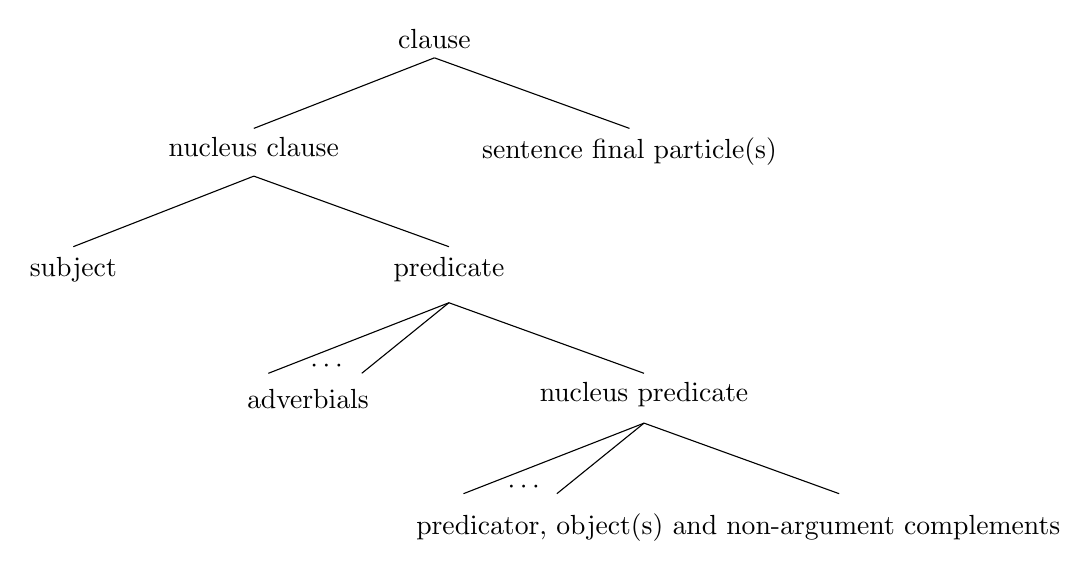
\begin{tikzpicture}[x=0.75pt,y=0.75pt,yscale=-1,xscale=1]
%uncomment if require: \path (0,383); %set diagram left start at 0, and has height of 383

%Straight Lines [id:da03870203201071365] 
\draw    (306,64.48) -- (219,98.48) ;
%Straight Lines [id:da09410121434078333] 
\draw    (306,64.48) -- (400,98.48) ;
%Straight Lines [id:da6473752338850502] 
\draw    (219,121.48) -- (132,155.48) ;
%Straight Lines [id:da22452164165522825] 
\draw    (219,121.48) -- (313,155.48) ;
%Straight Lines [id:da12042747516750363] 
\draw    (313,182.48) -- (226,216.48) ;
%Straight Lines [id:da6837235841990796] 
\draw    (313,182.48) -- (407,216.48) ;
%Straight Lines [id:da3234320748825805] 
\draw    (313,182.48) -- (271,216.48) ;
%Straight Lines [id:da4586272779304892] 
\draw    (407,240.48) -- (320,274.48) ;
%Straight Lines [id:da815197318792398] 
\draw    (407,240.48) -- (501,274.48) ;
%Straight Lines [id:da0031789117644716036] 
\draw    (407,240.48) -- (365,274.48) ;

% Text Node
\draw (306,61.48) node [anchor=south] [inner sep=0.75pt]   [align=left] {clause};
% Text Node
\draw (400,101.48) node [anchor=north] [inner sep=0.75pt]   [align=left] {sentence final particle(s)};
% Text Node
\draw (219,101.48) node [anchor=north] [inner sep=0.75pt]   [align=left] {nucleus clause};
% Text Node
\draw (132,159.48) node [anchor=north] [inner sep=0.75pt]   [align=left] {subject};
% Text Node
\draw (313,159.48) node [anchor=north] [inner sep=0.75pt]   [align=left] {predicate};
% Text Node
\draw (245,209) node [anchor=north west][inner sep=0.75pt]   [align=left] {$\displaystyle \cdots $};
% Text Node
\draw (207,223) node [anchor=north west][inner sep=0.75pt]   [align=left] {\begin{minipage}[lt]{55.17pt}\setlength\topsep{0pt}
\begin{center}
adverbials
\end{center}

\end{minipage}};
% Text Node
\draw (407,219.48) node [anchor=north] [inner sep=0.75pt]   [align=left] {nucleus predicate};
% Text Node
\draw (340,267) node [anchor=north west][inner sep=0.75pt]   [align=left] {$\displaystyle \cdots $};
% Text Node
\draw (296,283) node [anchor=north west][inner sep=0.75pt]   [align=left] {predicator, object(s) and non-argument complements};


\end{tikzpicture}

    \caption{The School Grammar analysis of clause structure}
    \label{fig:school-grammar-clause}
\end{figure}

\prettyref{fig:school-grammar-clause} is more about syntactic functions than the inner structure of constituents.
% TODO:不同位置可以填充什么成分

\section{The nucleus predicate}

The constituent order in the nucleus predicate is the follows:
\begin{exe}
    \ex 
\end{exe}

\section{Negation}

There is no negative concord in Chinese, 
but there is no uniform negation operator like the English \emph{not} in Chinese, either. 

\begin{exe}
    \ex \begin{xlist}
        \ex 我做 [不了]_{\text{potential complement, negative}} 这件事。
        \ex[*]{我\{没有/并非/不\}_{\text{negative operator}} 做 [得了]_{\text{potential complement, positive}} 这件事。}
    \end{xlist}    
\end{exe}

% TODO:句子中的全局依赖全部放到这里

\end{document}